%--- Cover slide will be handled by \titlepage in keynote.tex ---

%--- Slide 1: Outline ---
\begin{refsection}
  \begin{frame}{Outline}
    \begin{itemize}
      \item Generative Models and Diffusion Methods
      \item Applications in Remote Sensing and Synthetic Data
      \item Project Assignment
    \end{itemize}
  \end{frame}
\end{refsection}

\begin{refsection}
\begin{frame}{Generative Modeling}
  \begin{figure}
    \centering
    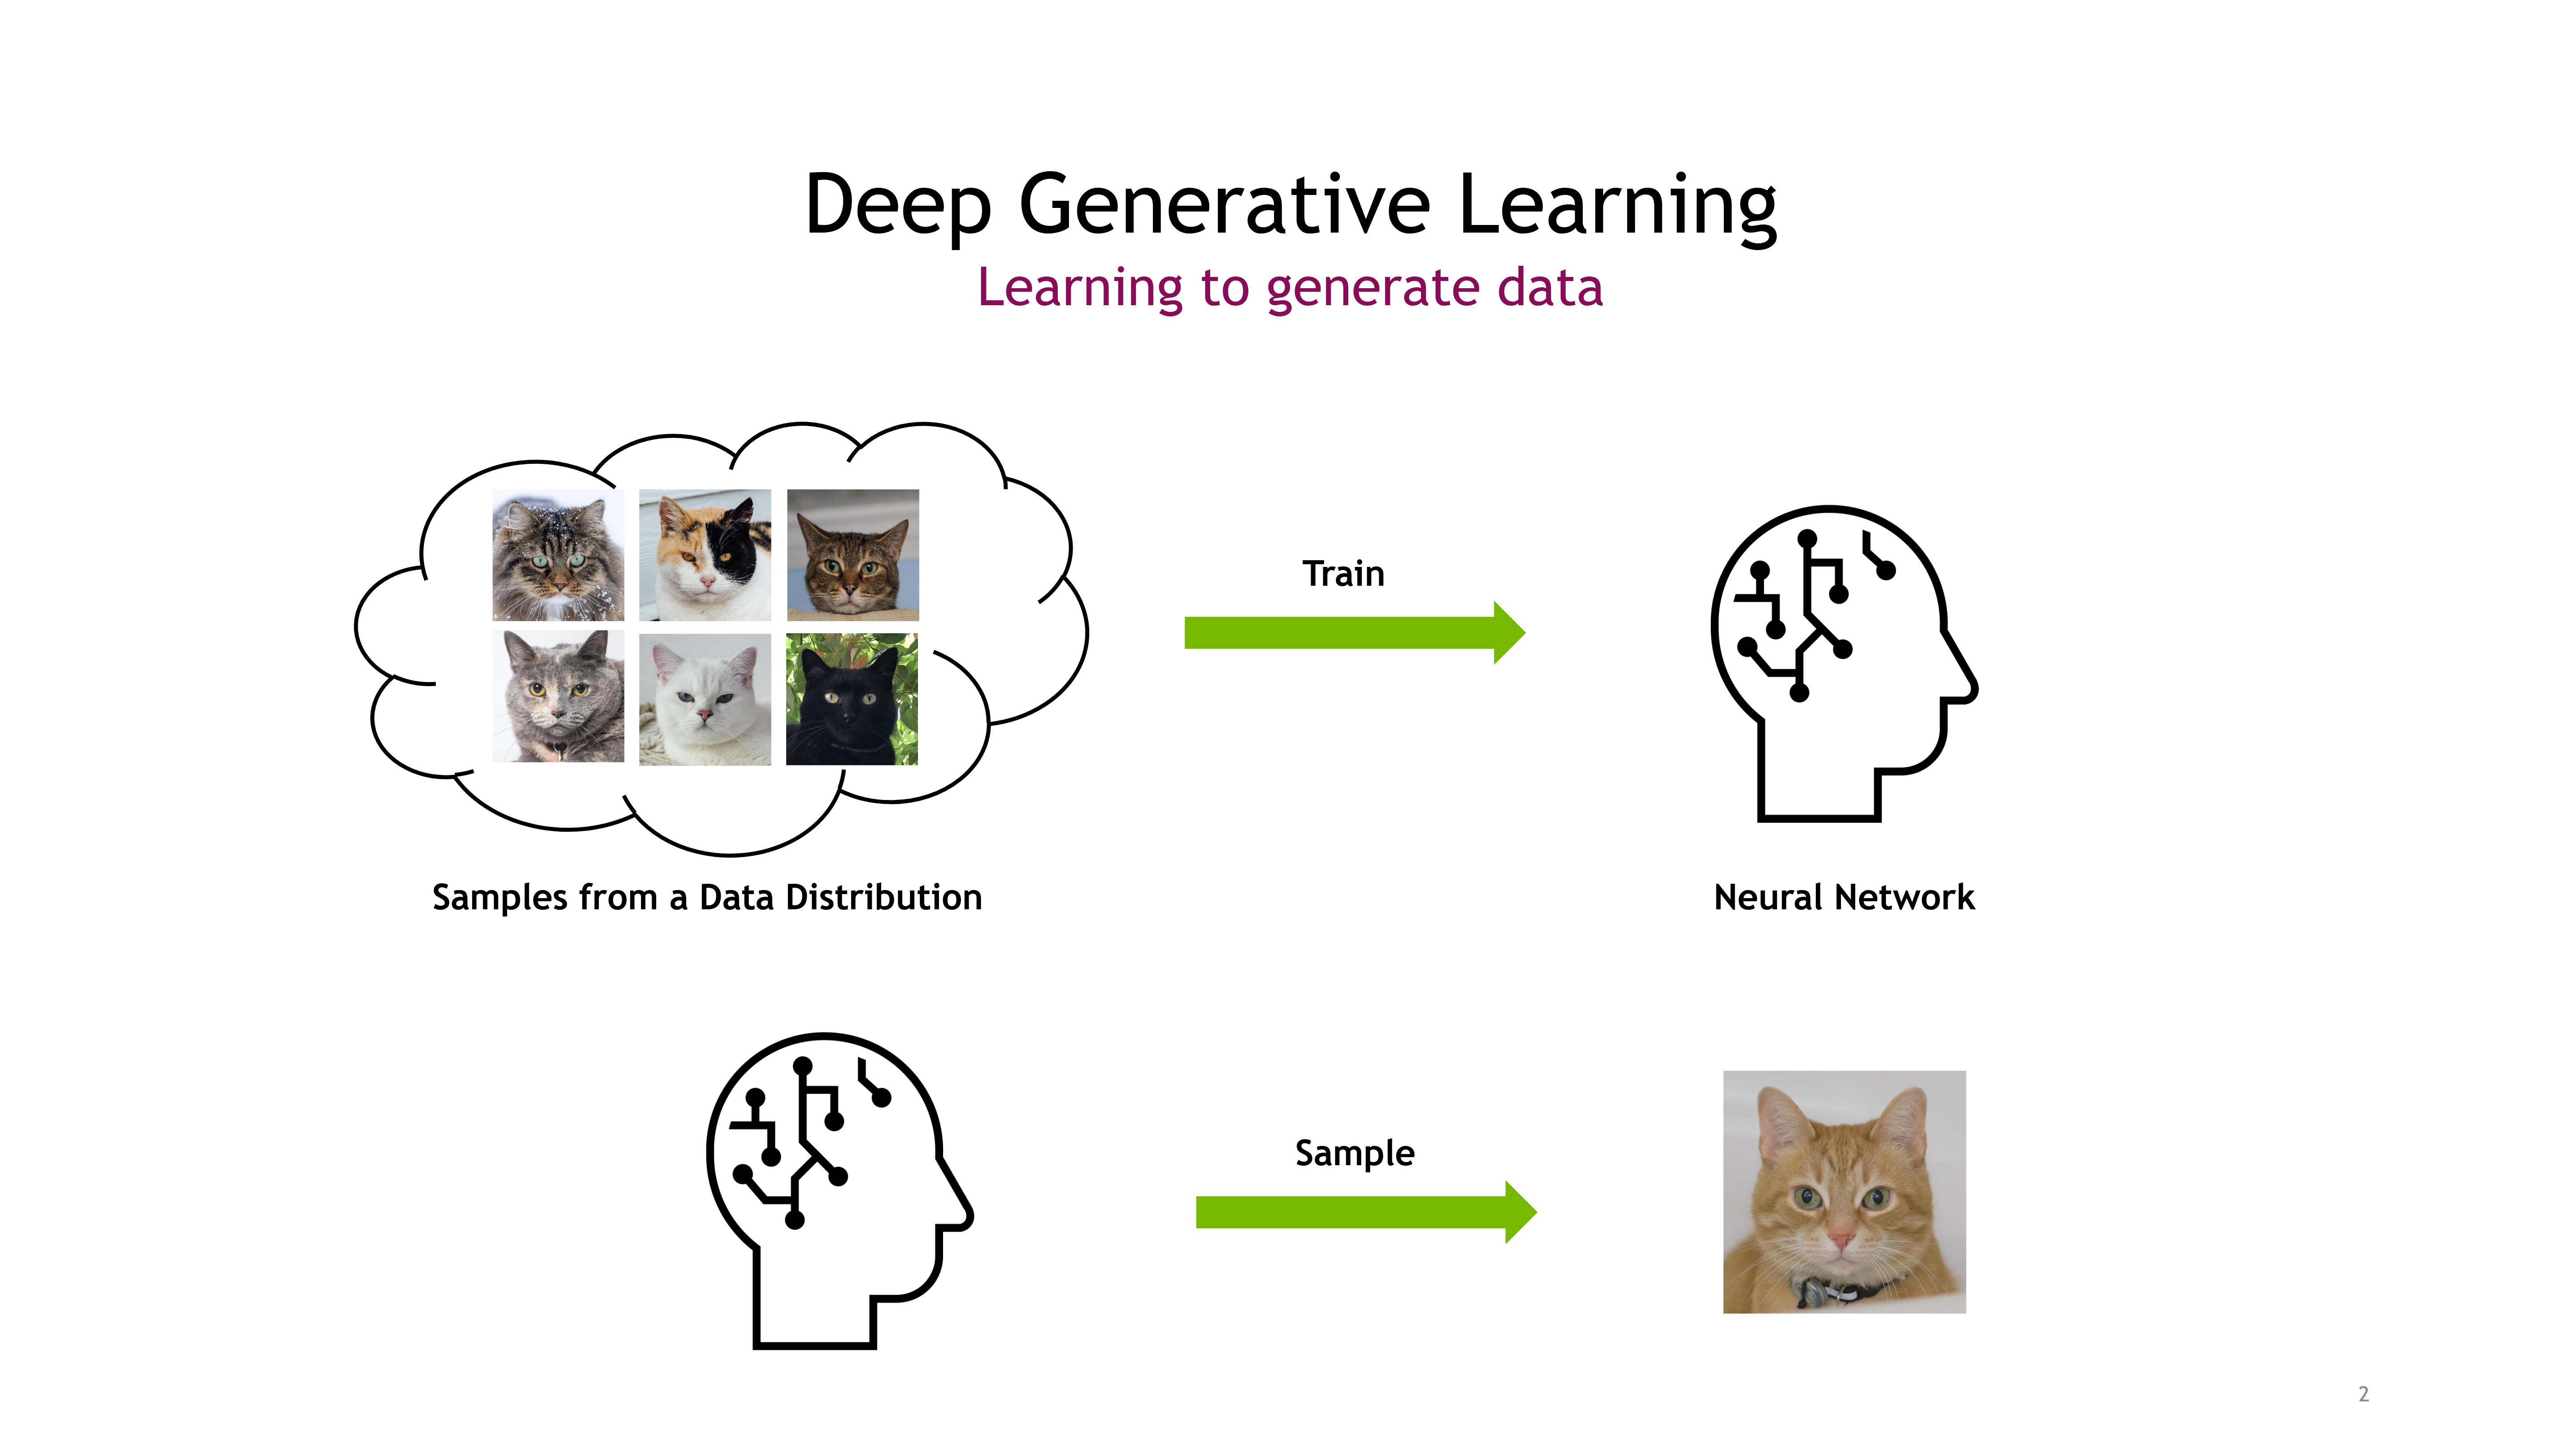
\includegraphics[width=0.8\linewidth]{figs/learning_to_generate_data.png}
    \caption{\scriptsize Illustration of generative modeling~\parencite{CVPR2023Tutorial}.}
  \end{figure}
  \bottomleftrefs
\end{frame}
\end{refsection}

% --- Slide 2: Timeline of Generative Models ---
\begin{refsection}
\begin{frame}{Timeline of Generative Models}
  \begin{figure}
    \centering
    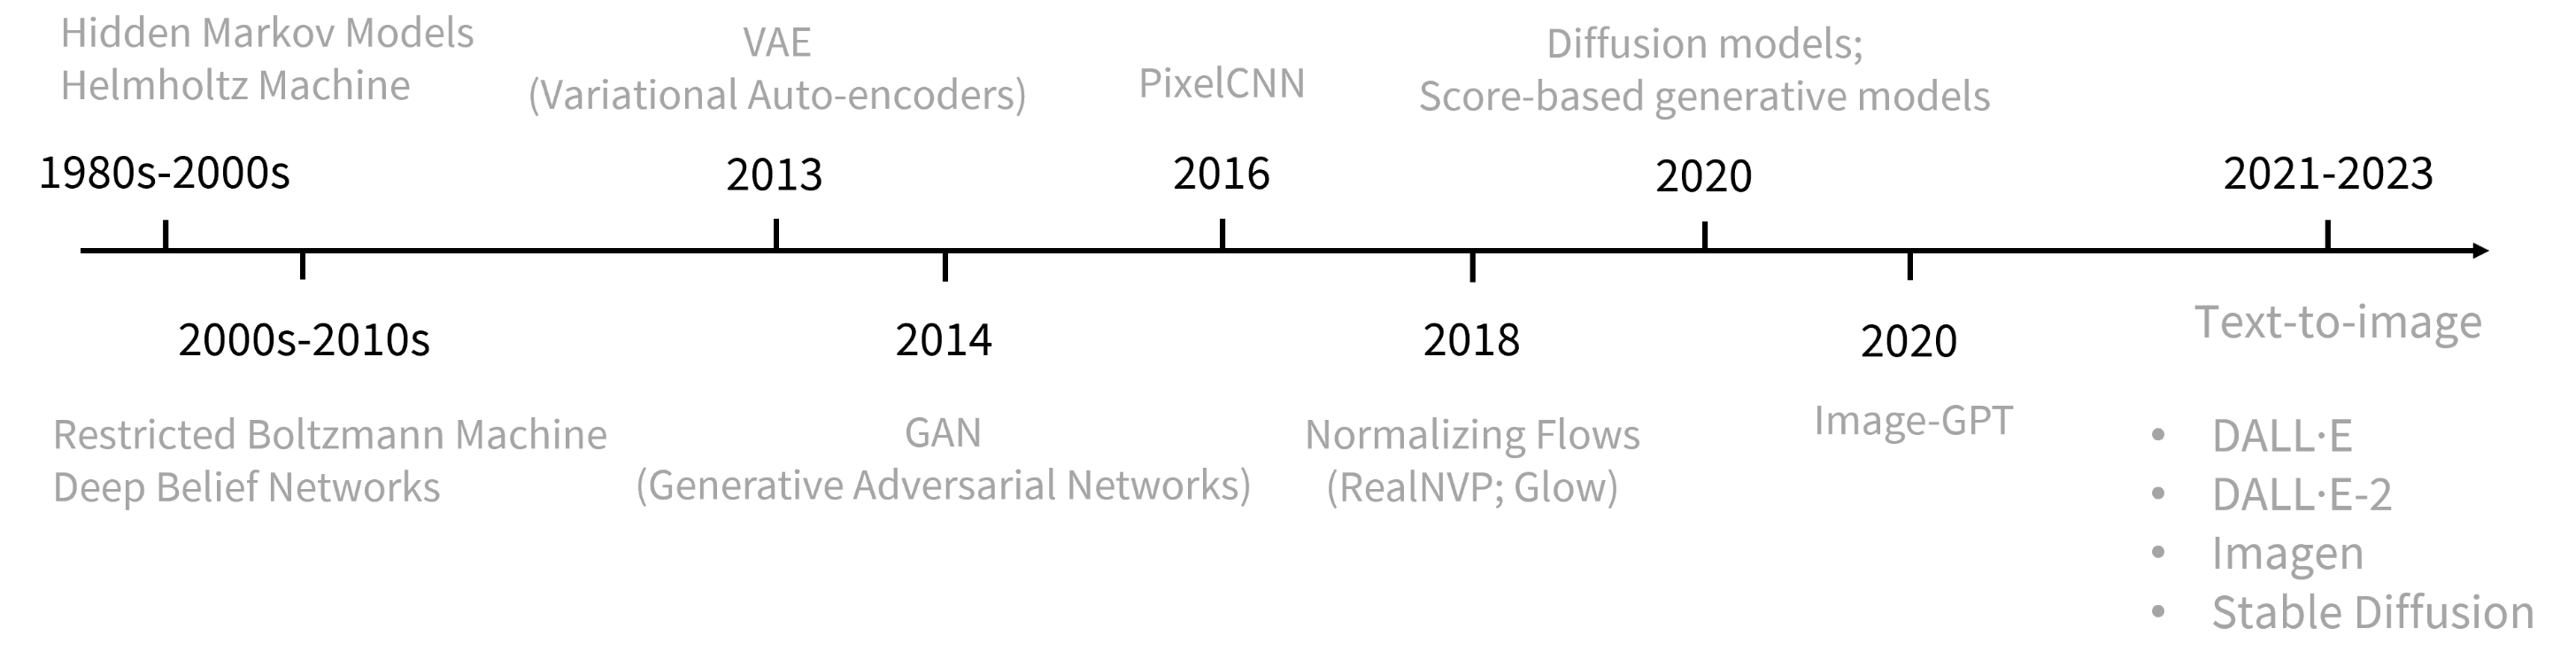
\includegraphics[width=0.95\linewidth]{figs/genai_timeline.png}
    \caption{\scriptsize Timeline of key developments in generative models~\parencite{dengPPTAdvancedNueralNetwork2024}.}
  \end{figure}
  \bottomleftrefs
\end{frame}
\end{refsection}



\begin{refsection}
\begin{frame}{Background: Diffusion Models}

  \begin{figure}
    \begin{minipage}{0.95\linewidth}
      \footnotesize
      \textbf{Denoising diffusion models consist of two processes:}
      \begin{itemize}
        \item A forward diffusion process that gradually adds noise to the input.
        \item A reverse denoising process that learns to generate data by denoising.
      \end{itemize}
    \end{minipage}
    \vspace{2em}

    \centering
    \includegraphics[width=1.0\linewidth]{figs/diffusion_high_level.png}

    \caption[]{\scriptsize Diffusion models generate data through iterative denoising~\parencite{sohl2015deep,ho2020denoising}.}
  \end{figure}

  \bottomleftrefs
\end{frame}
\end{refsection}

% --- Slide 4: Preliminaries of Diffusion Models ---
\begin{refsection}
\begin{frame}{Diffusion Models: Forward and Reverse Processes}
  \footnotesize
  \textbf{Forward (Diffusion) Process:}
  \begin{align*}
    q(\mathbf{x}_t \mid \mathbf{x}_{t-1}) &= \mathcal{N}(\mathbf{x}_t; \sqrt{1-\beta_t}\,\mathbf{x}_{t-1}, \beta_t \mathbf{I}) \\
    q(\mathbf{x}_{1:T} \mid \mathbf{x}_0) &= \prod_{t=1}^T q(\mathbf{x}_t \mid \mathbf{x}_{t-1}) \\
    &\text{Equivalently,  } 
    \mathbf{x}_t = \sqrt{\bar{\alpha}_t}\,\mathbf{x}_0 + \sqrt{1-\bar{\alpha}_t}\,\boldsymbol{\epsilon}, \quad \boldsymbol{\epsilon} \sim \mathcal{N}(\mathbf{0}, \mathbf{I})
  \end{align*}

  \footnotesize
  \textbf{Reverse (Denoising) Process:}
  \begin{align*}
    p_\theta(\mathbf{x}_{t-1} \mid \mathbf{x}_t) &= \mathcal{N}(\mathbf{x}_{t-1}; \boldsymbol{\mu}_\theta(\mathbf{x}_t, t), \Sigma_\theta(\mathbf{x}_t, t)) \\
    p_\theta(\mathbf{x}_{0:T}) &= p(\mathbf{x}_T) \prod_{t=1}^T p_\theta(\mathbf{x}_{t-1} \mid \mathbf{x}_t)
  \end{align*}
  \scriptsize
  where $\mathbf{x}_0$ is the data, $\beta_t$ is the noise schedule, and $\bar{\alpha}_t = \prod_{s=1}^t (1-\beta_s)$. $p(\mathbf{x}_T) = \mathcal{N}(\mathbf{0}, \mathbf{I})$.

  \scriptsize
  \textbf{Diffusion models generate data by learning to reverse a gradual noising process.}~\parencite{sohl2015deep,ho2020denoising}
  \bottomleftrefs
\end{frame}
\end{refsection}

\begin{refsection}
\begin{frame}{Diffusion Models: Training and Inference}
  \footnotesize
  \textbf{Training Objective:}
  \begin{align*}
    \mathcal{L}_{\mathrm{simple}} = \mathbb{E}_{\mathbf{x}_0, \boldsymbol{\epsilon}, t} \left[ \left\| \boldsymbol{\epsilon} - \boldsymbol{\epsilon}_\theta(\sqrt{\bar{\alpha}_t}\mathbf{x}_0 + \sqrt{1-\bar{\alpha}_t}\boldsymbol{\epsilon}, t) \right\|^2 \right]
  \end{align*}
  where $\boldsymbol{\epsilon} \sim \mathcal{N}(\mathbf{0}, \mathbf{I})$, $\bar{\alpha}_t = \prod_{s=1}^t (1-\beta_s)$.

  \vspace{0.5em}
  \textbf{Inference (Sampling):}
  \begin{itemize}
    \item Start from pure noise: $\mathbf{x}_T \sim \mathcal{N}(\mathbf{0}, \mathbf{I})$
    \item For $t = T, \ldots, 1$:
      \begin{itemize}
        \item Predict noise: $\boldsymbol{\epsilon}_\theta(\mathbf{x}_t, t)$
        \item Compute mean: $\boldsymbol{\mu}_\theta(\mathbf{x}_t, t)$
        \item Sample: $\mathbf{x}_{t-1} \sim \mathcal{N}(\boldsymbol{\mu}_\theta(\mathbf{x}_t, t), \Sigma_\theta(\mathbf{x}_t, t))$
      \end{itemize}
    \item Repeat until $\mathbf{x}_0$ (generated sample)
  \end{itemize}

  \vspace{0.5em}
  \scriptsize
  \textbf{Training:} Minimize the simplified objective~\parencite{ho2020denoising}.\\
  \textbf{Inference:} Iteratively denoise from random noise to generate data.
  \bottomleftrefs
\end{frame}
\end{refsection}

%--- Slide 5: Application in Remote Sensing Image Generation: DiffusionSat, CRS-Diff, Text2Earth ---

\begin{refsection}
  \begin{frame}{Application in Remote Sensing Image Generation: Text2Earth}
    \begin{figure}
      \centering
      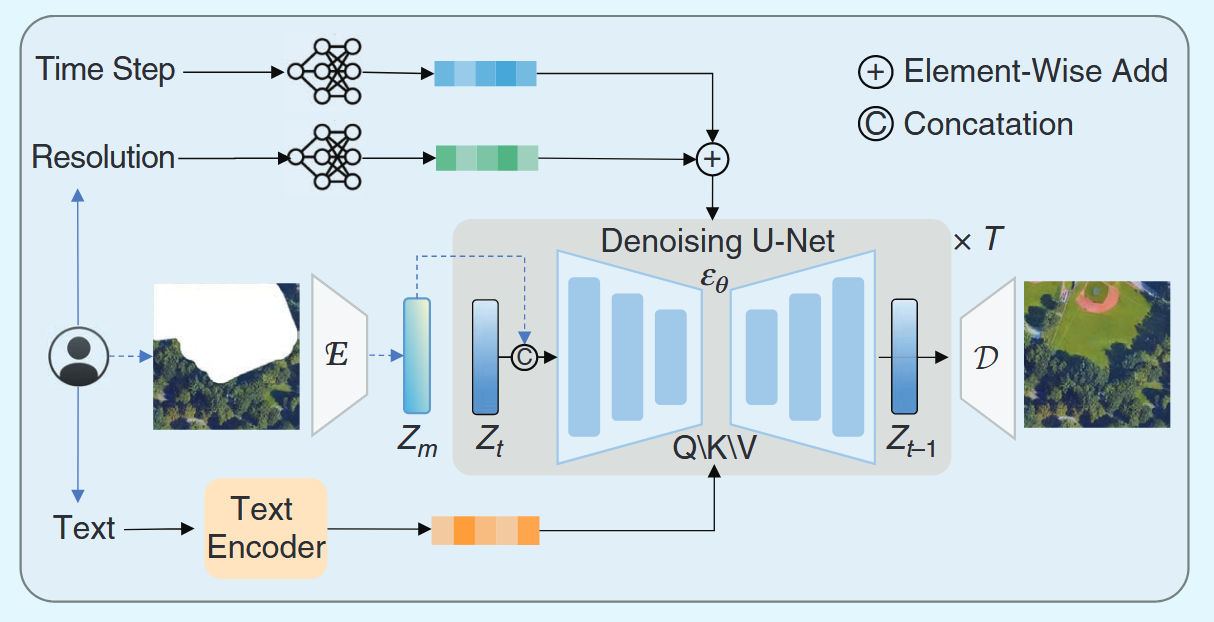
\includegraphics[width=0.9\linewidth]{figs/text2earth.png}
      \caption[]{\scriptsize Text2Earth: Foundation model for text-driven Earth observation~\parencite{text2earth2025}.}
    \end{figure}
    \bottomleftrefs
  \end{frame}
\end{refsection}

\begin{refsection}
  \begin{frame}{Text2Earth: Example Results}
    \begin{figure}
      \centering
      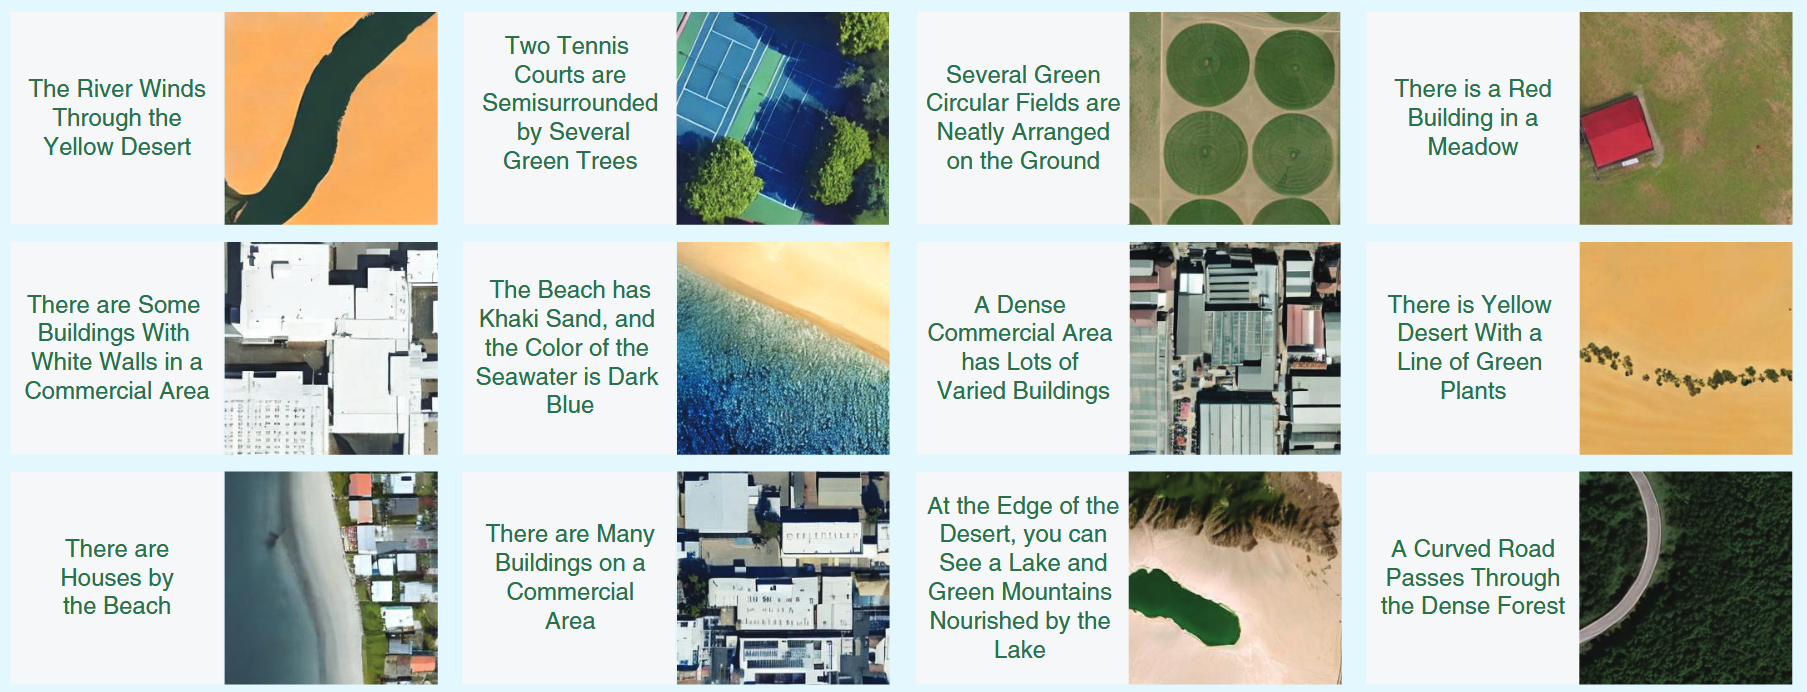
\includegraphics[width=0.9\linewidth]{figs/text2earth_results.png}
      \caption[]{\scriptsize Example results generated by Text2Earth~\parencite{text2earth2025}.}
    \end{figure}
    \bottomleftrefs
  \end{frame}
\end{refsection}

\begin{refsection}
\begin{frame}{Application in Remote Sensing Image Generation: CRS-Diff}
  \begin{figure}
    \centering
    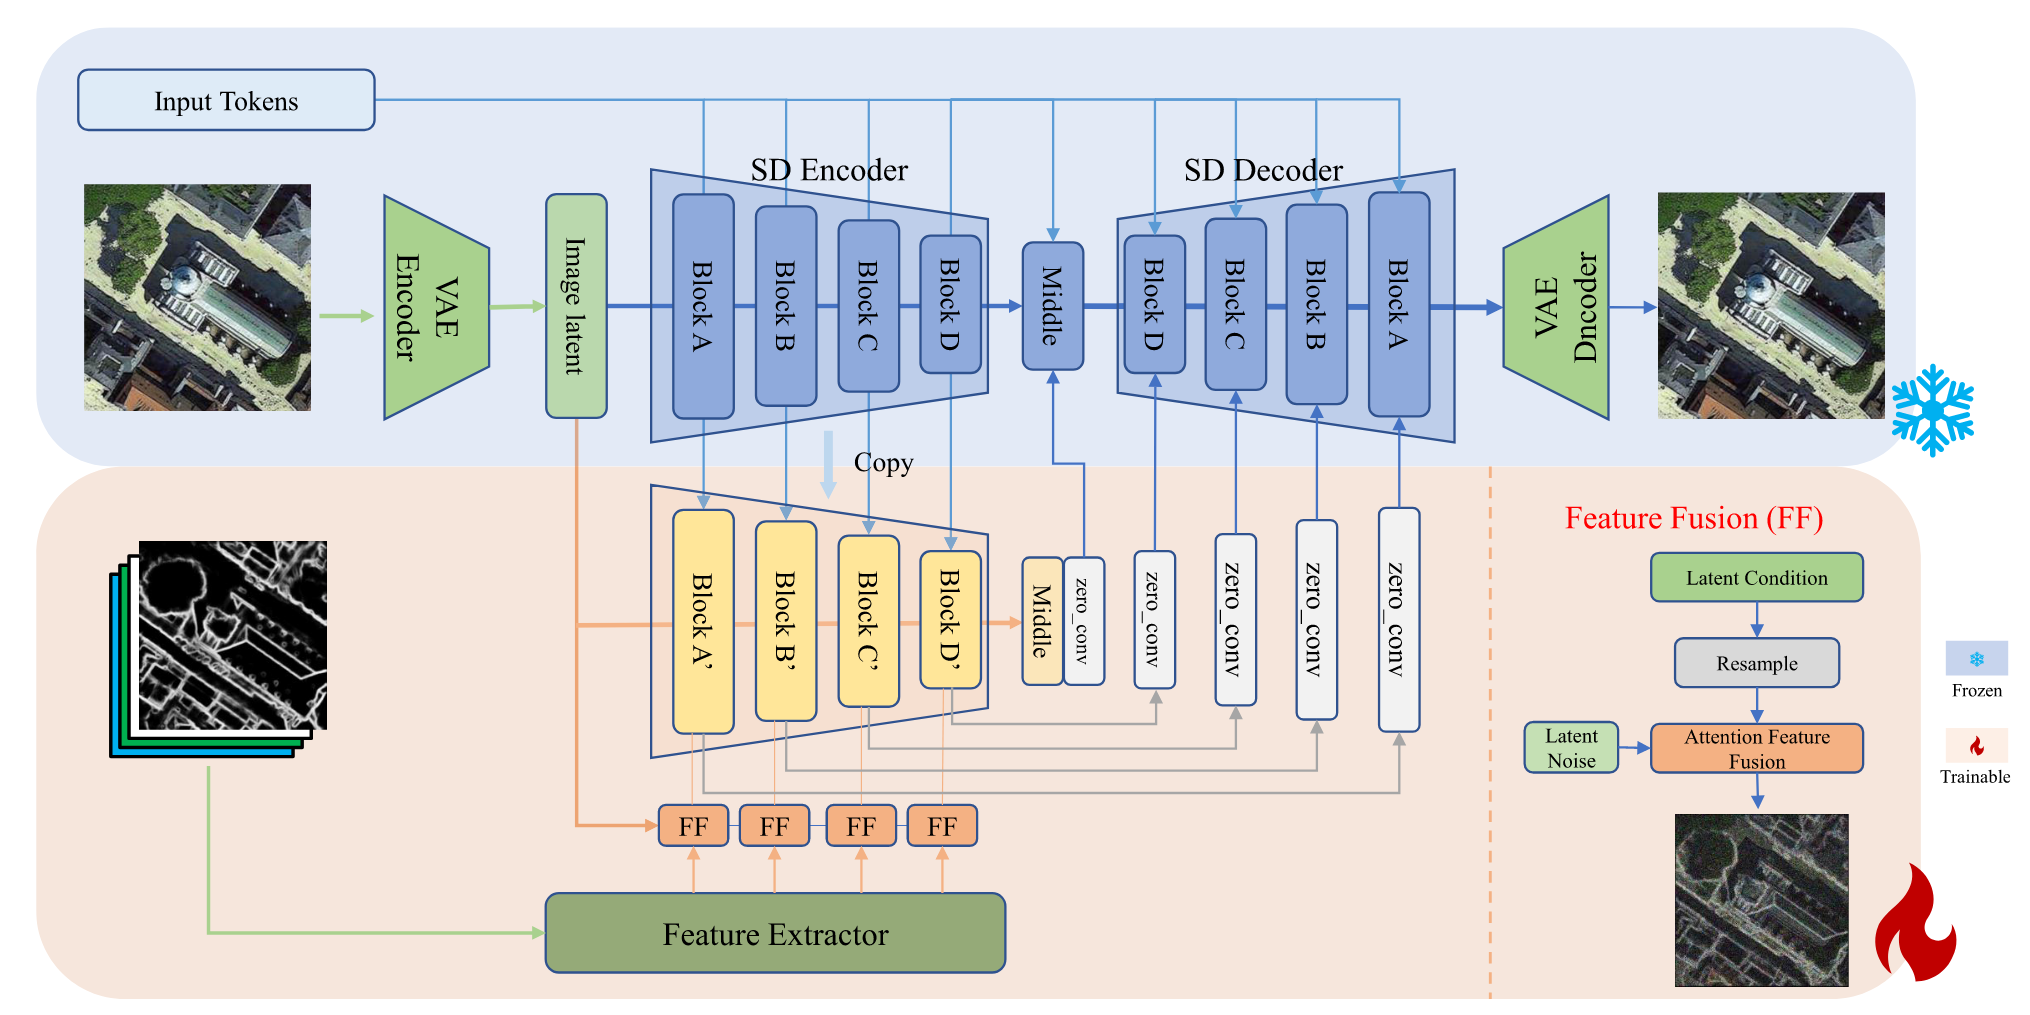
\includegraphics[width=0.9\linewidth]{figs/crsdiff.png}
    \caption[]{\scriptsize CRS-Diff: Controllable remote sensing image generation framework~\parencite{tang2024crsdiff}.}
  \end{figure}
  \bottomleftrefs
\end{frame}
\end{refsection}

\begin{refsection}
\begin{frame}{CRS-Diff: Example Results}
  \begin{figure}
    \centering
    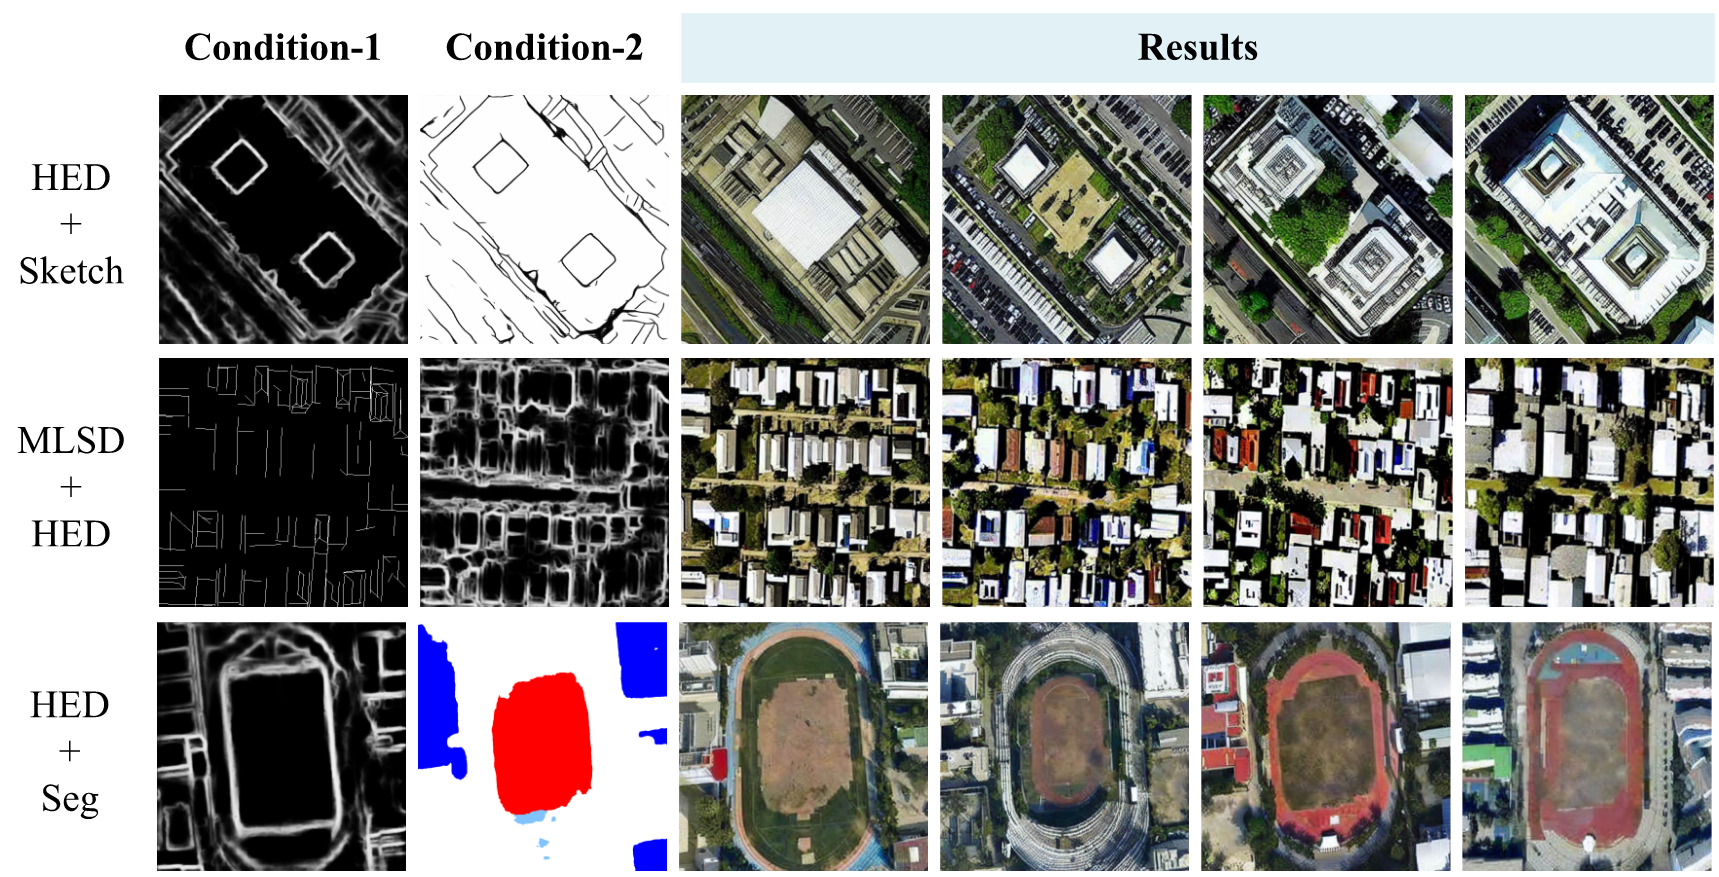
\includegraphics[width=0.9\linewidth]{figs/crsdiff_results.png}
    \caption[]{\scriptsize Example results generated by CRS-Diff~\parencite{tang2024crsdiff}.}
  \end{figure}
  \bottomleftrefs
\end{frame}
\end{refsection}


%--- Slide 6a: DiffusionSat Framework ---
\begin{refsection}
\begin{frame}{DiffusionSat: Framework Overview}
  \begin{figure}
    \centering
    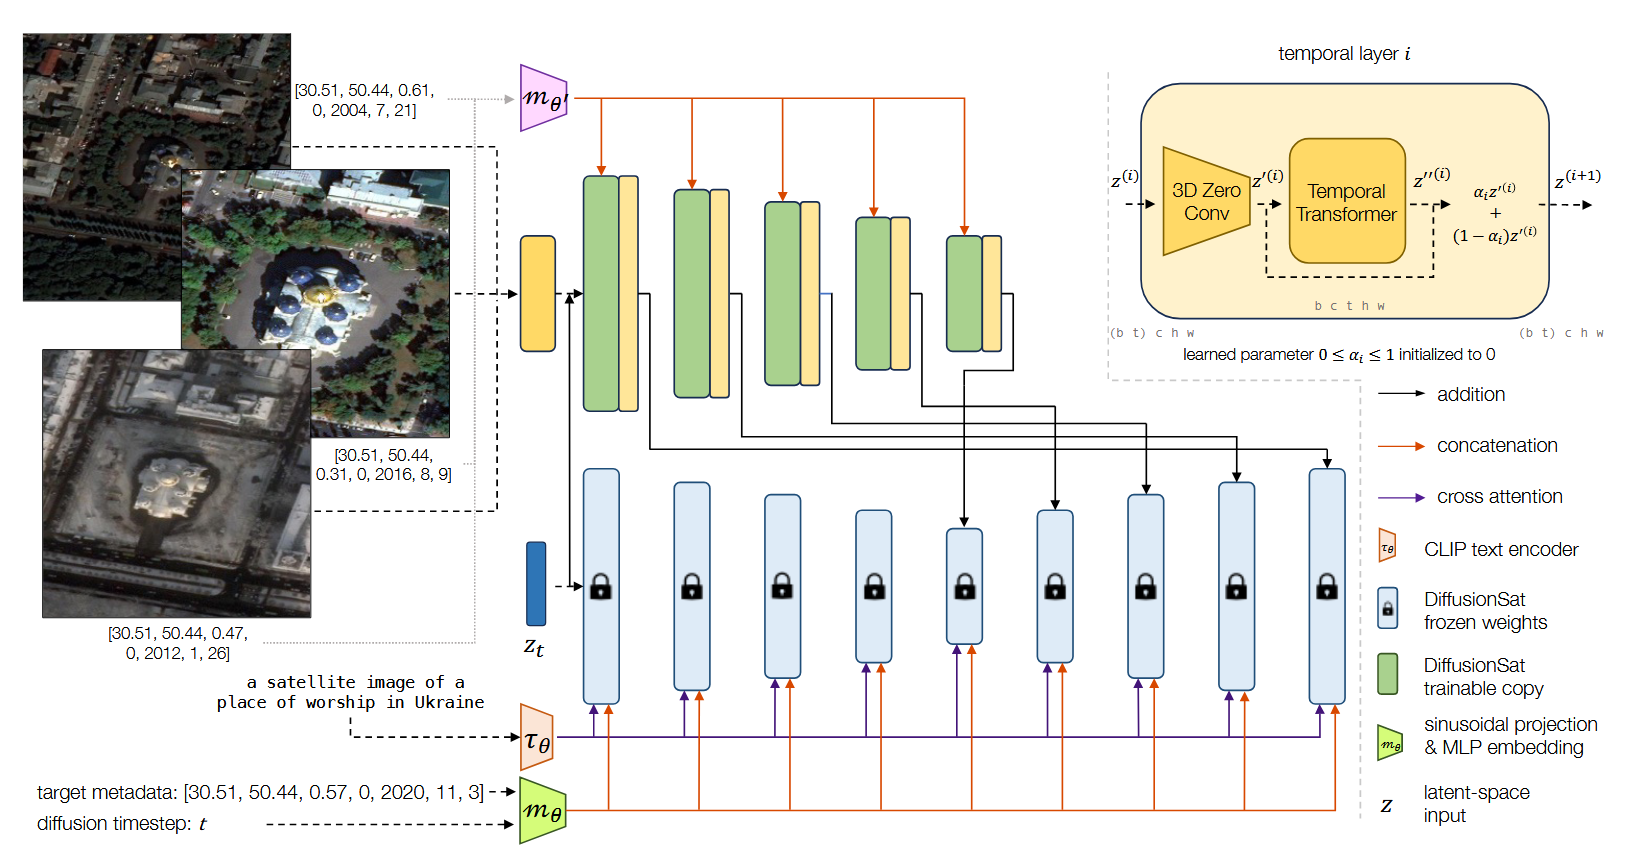
\includegraphics[width=0.9\linewidth]{figs/diffusionsat.png}
    \caption[]{\scriptsize DiffusionSat: A generative foundation model for satellite imagery~\parencite{diffusionset2024}.}
  \end{figure}
  \bottomleftrefs
\end{frame}
\end{refsection}

%--- Slide 6b: DiffusionSat for Super-Resolution ---
\begin{refsection}
\begin{frame}{DiffusionSat: Super-Resolution Results}
  \begin{figure}
    \centering
    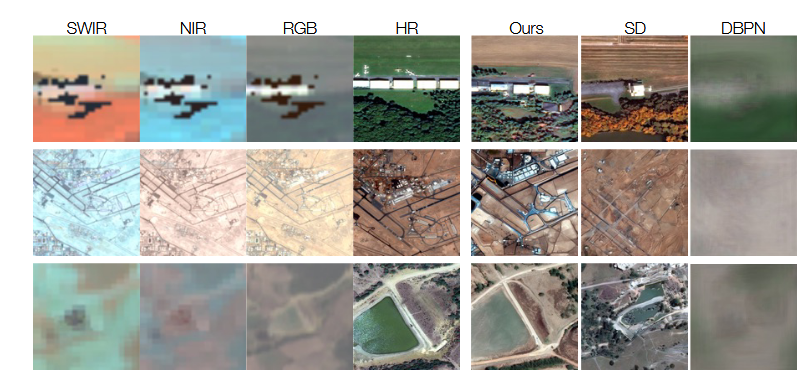
\includegraphics[width=0.9\linewidth]{figs/diffusionsat_sr_results.png}
    \caption[]{\scriptsize Example results: DiffusionSat for multi-spectral super-resolution~\parencite{diffusionset2024}.}
  \end{figure}
  \bottomleftrefs
\end{frame}
\end{refsection}

%--- Slide 6c: DiffusionSat for Inpainting ---
\begin{refsection}
\begin{frame}{DiffusionSat: Inpainting Results}
  \begin{figure}
    \centering
    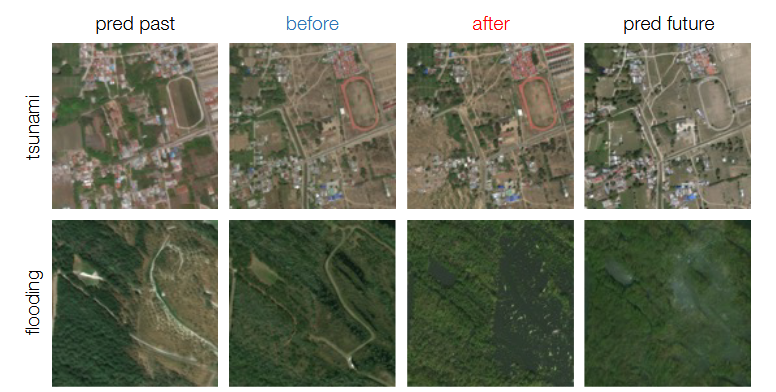
\includegraphics[width=0.9\linewidth]{figs/diffusionsat_inpainting_results.png}
    \caption[]{\scriptsize Example results: DiffusionSat for remote sensing image inpainting~\parencite{diffusionset2024}.}
  \end{figure}
  \bottomleftrefs
\end{frame}
\end{refsection}



%--- Slide 8: Q&A ---
\begin{refsection}
\begin{frame}[plain]
  \vfill
  \centering
  {\LARGE \textbf{Q\&A}}
  \vfill
\end{frame}
\end{refsection}

\begin{refsection}
  \begin{frame}{Project Assignment: Research Topic}
    \textbf{Main Question:} \\
    \vspace{0.5em}
    Is synthetic data from generative models ready for image recognition?
  
    \vspace{1em}
    \begin{itemize}
      \item Synthetic data generated by generative models is a trending new way of data augmentation~\parencite{heSYNTHETICDATAGENERATIVE2022,tokerSatSynthAugmentingImageMask2024}.
      \item In this project, we will explore whether such augmentation benefits downstream tasks such as text-image retrieval, image scene classification, and super-resolution in the remote sensing domain.
      % \item Analyze recent research and conduct your own experiments.
    \end{itemize}
    \bottomleftrefs
  \end{frame}
  \end{refsection}

  
\begin{refsection}
  \begin{frame}{Background: Why Synthetic Data?}
    \begin{itemize}
      \item Manual data collection and annotation is expensive and time-consuming.
      \item Synthetic data from generative models enables large-scale data augmentation.
      \item The effectiveness of synthetic data for downstream remote sensing tasks is under active investigation.
    \end{itemize}
    \begin{minipage}{0.5\linewidth}
      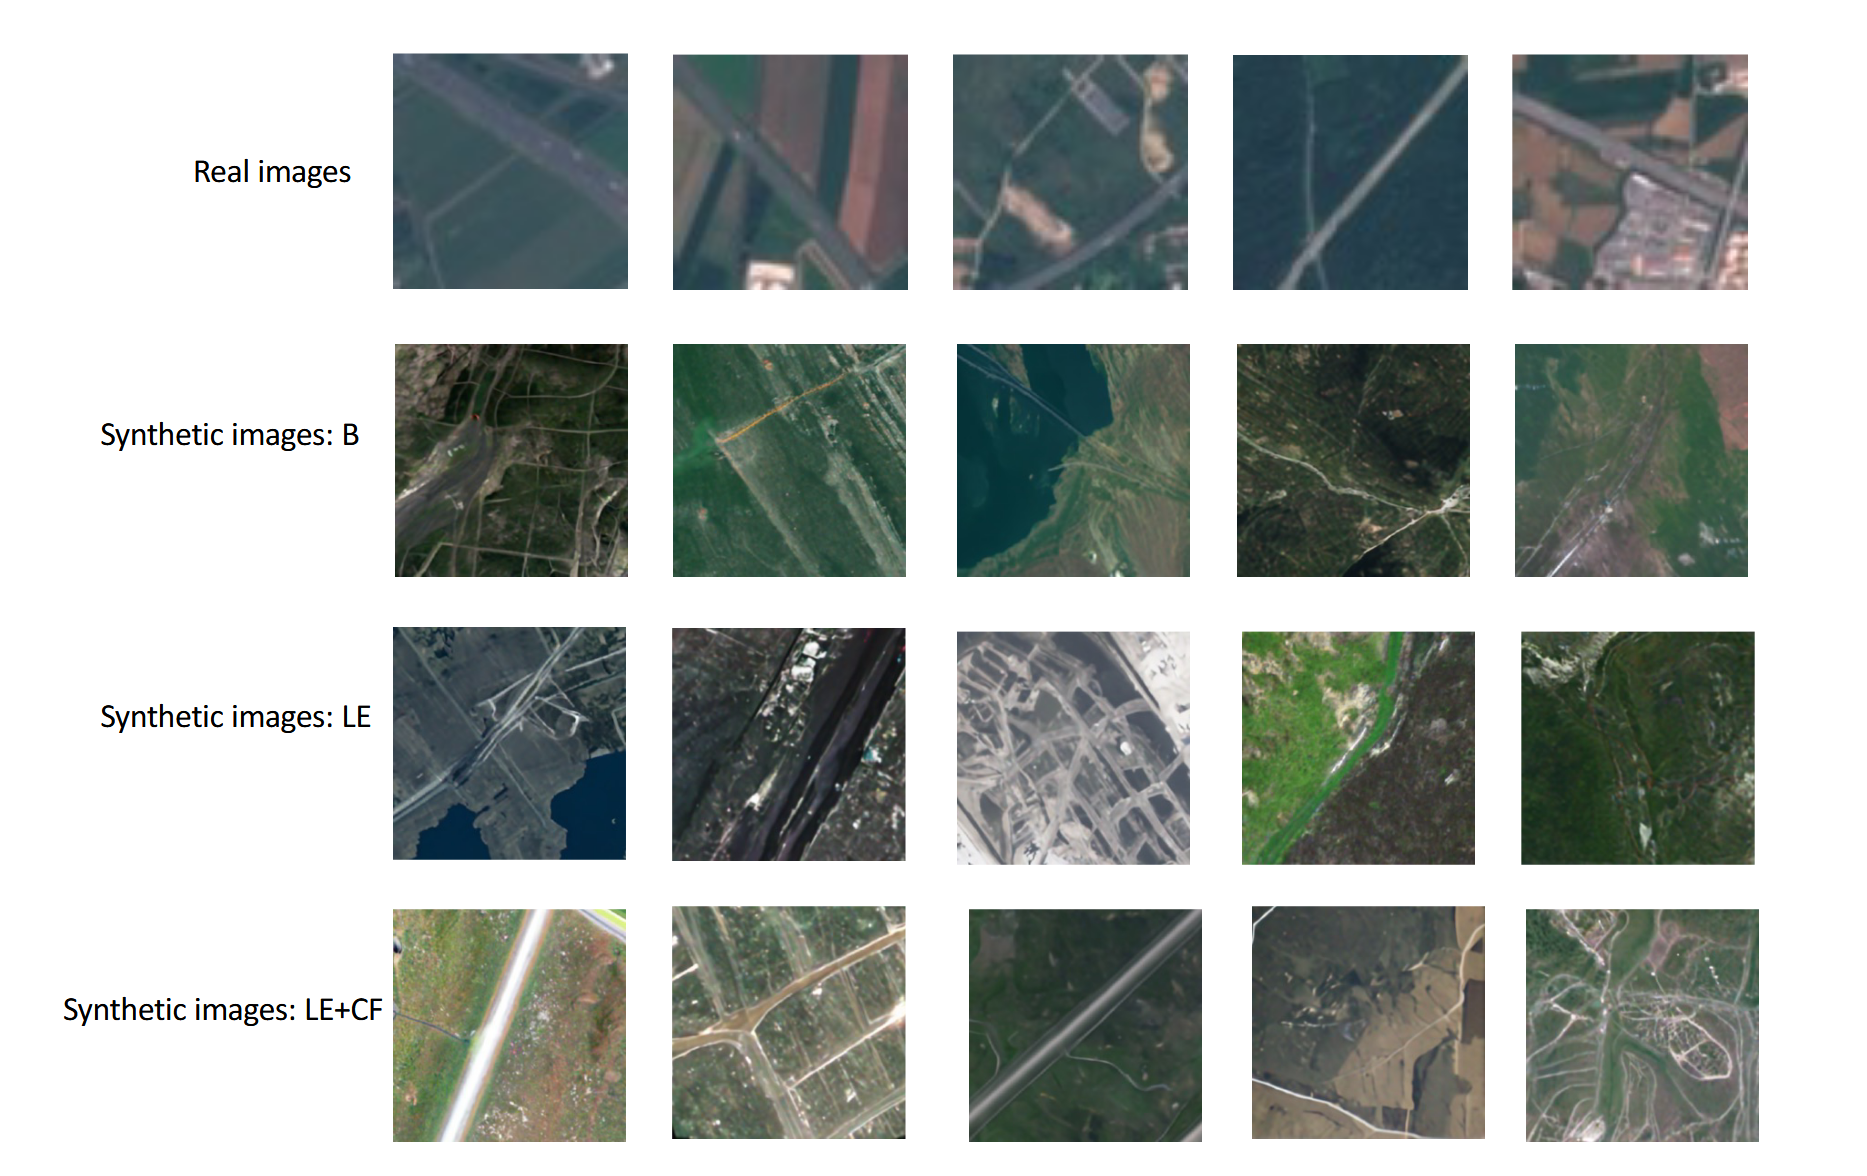
\includegraphics[width=\linewidth]{figs/Visualization_of_different_strategies_of_synthetic_data_in_zeroshot_settings.png}
    \end{minipage}%
    \hfill
    \begin{minipage}{0.4\linewidth}
      \vspace{0.5em}
      {\scriptsize
      \textbf{Visualization of different strategies of synthetic data in zero-shot settings~\parencite{heSYNTHETICDATAGENERATIVE2022}.} Visual illustration of ground-truth real data and synthesized images by different strategies for the zero-shot settings: basic (B), language enhancement (LE), and language enhancement with CLIP-based filtering (LE+CF).
      }
    \end{minipage}
    \bottomleftrefs
  \end{frame}
  \end{refsection}
  
  
  
  \begin{refsection}
    \begin{frame}{Experimental Settings: Generative Data for Downstream Tasks}
      \begin{itemize}
        \item We leverage state-of-the-art generative models such as \textbf{DiffusionSat}~\parencite{diffusionset2024} and \textbf{Text2Earth}~\parencite{text2earth2025} for synthetic data augmentation.
        \item \textbf{Two main strategies:}
        \begin{enumerate}
          \item \textbf{Text-to-image generation:}
            \begin{itemize}
              \item Generate text-image pairs.
              \item Enables tasks like image scene classification and image-text retrieval.
            \end{itemize}
          \item \textbf{Super-resolution generation:}
            \begin{itemize}
              \item Generate paired low-resolution (LR) and high-resolution (HR) images.
              \item Enables super-resolution tasks in remote sensing.
            \end{itemize}
        \end{enumerate}
      \end{itemize}
      \vspace{1em}
      % \begin{figure}
      %   \centering
      %   \fbox{\rule{0pt}{2in} \rule{0.8\linewidth}{0pt}} % Empty figure placeholder
      %   \caption{\scriptsize Experimental pipeline: Synthetic data generation for downstream remote sensing tasks.}
      % \end{figure}
      \bottomleftrefs
    \end{frame}
    \end{refsection}

    %--- Additional Slides: Downstream Tasks for Project Assignment ---

% \begin{refsection}
%   \begin{frame}{Downstream Tasks Overview}
%     \begin{itemize}
%       \item In this project, we focus on two key downstream tasks:
%       \begin{enumerate}
%         \item \textbf{Image Scene Classification} using foundation models like CLIP.
%         \item \textbf{Image Super-Resolution} using generative models like Real-ESRGAN.
%       \end{enumerate}
%       \item We aim to evaluate whether synthetic data improves model performance on these tasks.
%     \end{itemize}
%   \end{frame}
%   \end{refsection}
  
  \begin{refsection}
  \begin{frame}{Image Scene Classification with CLIP}
    % \textbf{CLIP: Contrastive Language–Image Pretraining}
    \begin{figure}
      \centering
      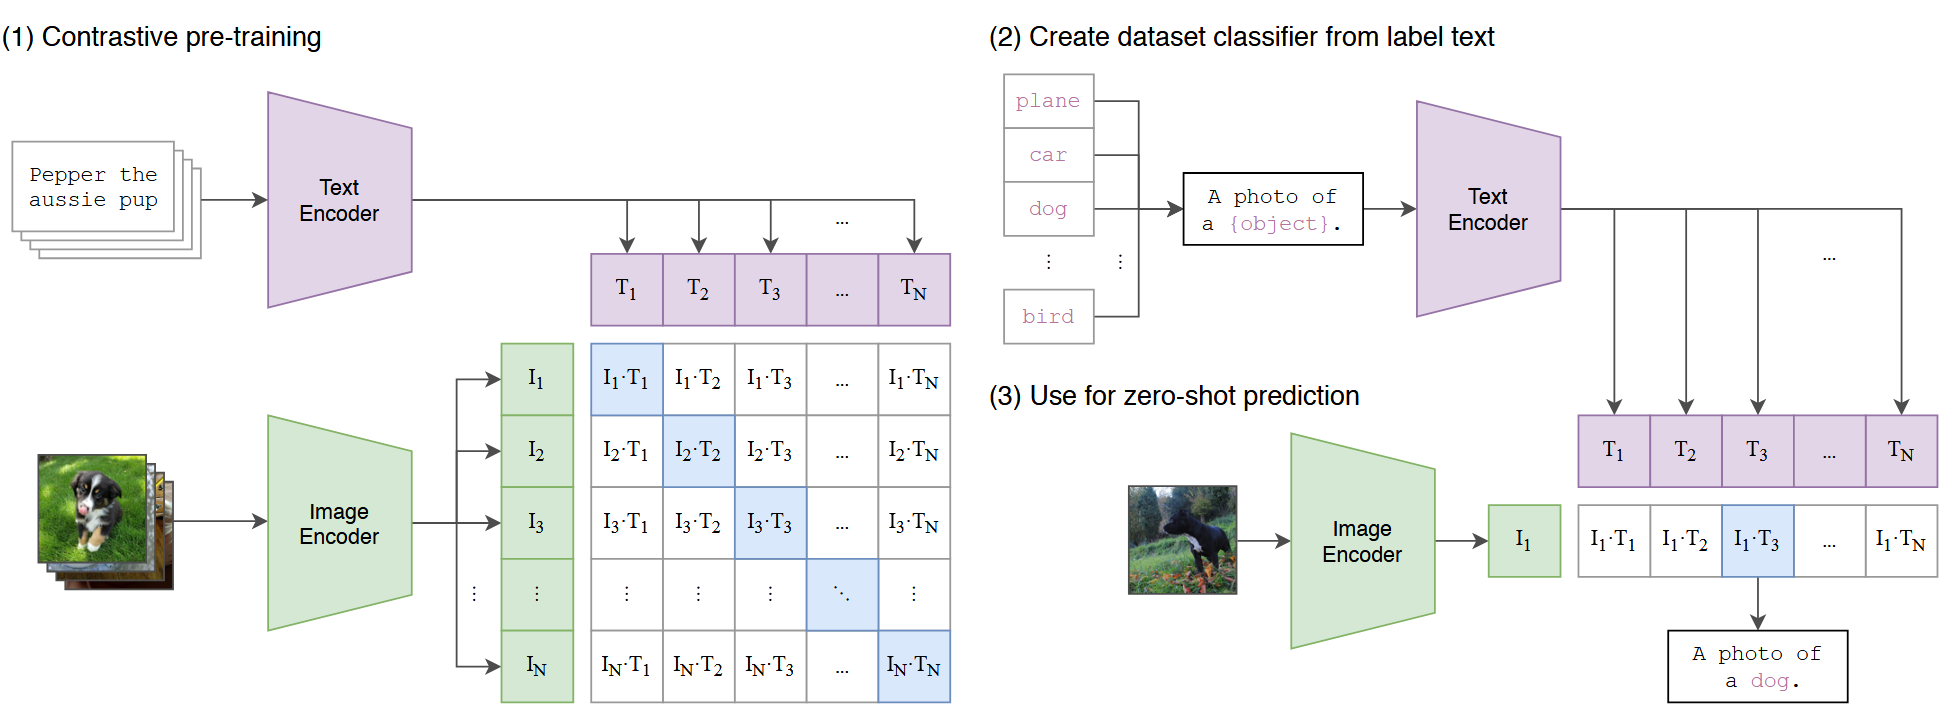
\includegraphics[width=\linewidth]{figs/clip.png}
      \caption{\scriptsize CLIP~\parencite{radfordLearningTransferableVisual2021} model overview: joint training of image and text encoders for cross-modal understanding.}
    \end{figure}

    \bottomleftrefs
  \end{frame}
  \end{refsection}
  
  \begin{refsection}
  \begin{frame}{Super-Resolution with Real-ESRGAN}
    % \textbf{Real-ESRGAN: Enhanced Super-Resolution GAN}
    \begin{figure}
      \centering
      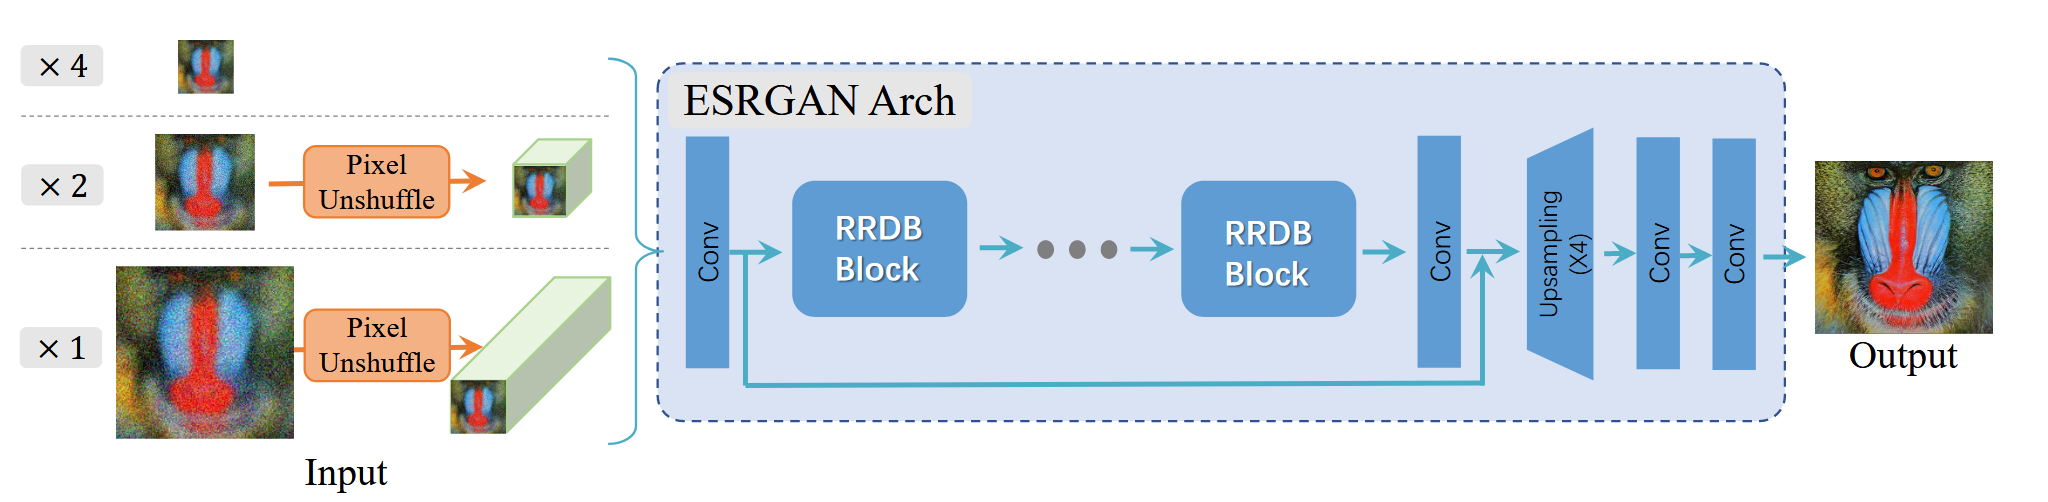
\includegraphics[width=\linewidth]{figs/realesrgan.png}
      \caption{\scriptsize Real-ESRGAN~\parencite{wangRealESRGANTrainingRealWorld2021b} framework: architecture for real-world image super-resolution.}
    \end{figure}
    \bottomleftrefs
  \end{frame}
  \end{refsection}

  
\begin{refsection}
  \begin{frame}{Baseline Models for Scene Classification and Super-Resolution}
    \textbf{Scene Image Classification:}
    \begin{itemize}
      \item \textbf{CLIP}~\parencite{radfordLearningTransferableVisual2021}
      \item \textbf{RemoteCLIP}~\parencite{liuRemoteCLIPVisionLanguage2024}
      \item \textbf{Git-RSCLIP}~\parencite{text2earth2025}
    \end{itemize}
    \textbf{Super-Resolution:}
    \begin{itemize}
      \item \textbf{Real-ESRGAN}~\parencite{wangRealESRGANTrainingRealWorld2021b}
      \item \textbf{StableSR}~\parencite{wangExploitingDiffusionPrior2024}
      \item \textbf{FaithDiff}~\parencite{chenFaithDiffUnleashingDiffusion2024}
      \item \textbf{EResShift}~\parencite{yueEfficientDiffusionModel2025}
    \end{itemize}
    % \begin{figure}
    %   \centering
    %   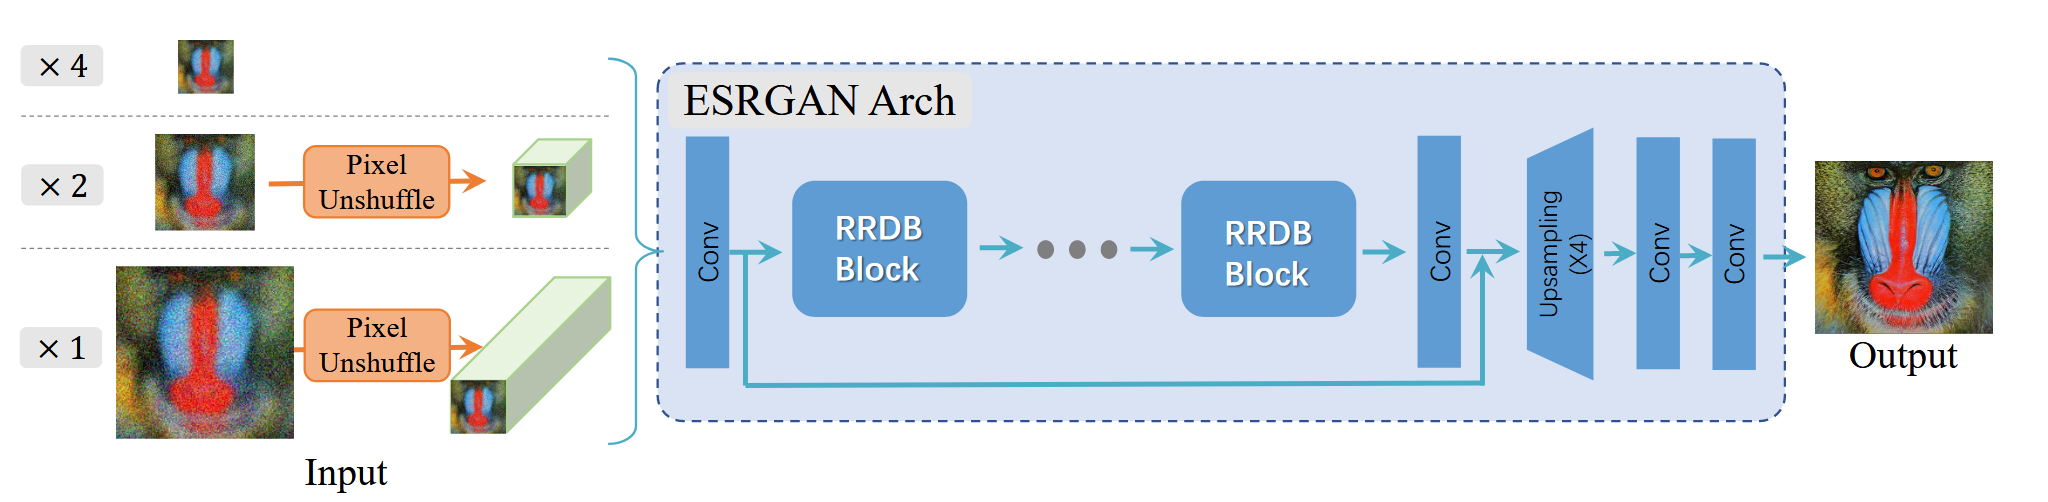
\includegraphics[width=0.7\linewidth]{figs/realesrgan.png}
    %   \caption{\scriptsize Real-ESRGAN framework.}
    % \end{figure}
    \bottomleftrefs
  \end{frame}
  \end{refsection}

  %--- Slide: Datasets for Text-to-Image Generation ---
\begin{refsection}
  \begin{frame}{Datasets for Text-to-Image Generation}
    \textbf{Text-to-Image Generation:}
    \begin{itemize}
      \item \textbf{RSICD}~\parencite{lu2017exploring}: Remote Sensing Image Captioning Dataset with 10,921 images and five captions per image.
      \item \textbf{RSICap}~\parencite{hu2023rsgpt}: High-quality dataset with 2,585 human-annotated image-caption pairs.
      \item \textbf{UCM-Captions}~\parencite{qu2016deep}: Derived from the UC Merced Land Use Dataset, containing 2,100 images with five captions each.
    \end{itemize}
    \bottomleftrefs
  \end{frame}
\end{refsection}

%--- Slide: Datasets for Super-Resolution ---
\begin{refsection}
  \begin{frame}{Datasets for Super-Resolution}
    \textbf{Super-Resolution:}
    \begin{itemize}
      \item \textbf{fMoW}: Paired dataset of Sentinel-2 (10m GSD)~\parencite{congFunctionalMapWorld2022} and fMoW-RGB (0.3m)~\parencite{christieFunctionalMapWorld2018}.
      \item 22,852 high-resolution RSIs (256 × 256 size) used in~\parencite{mengConditionalDiffusionModel2024} from Potsdam from the ISPRS 2-D semantic labeling contest~\parencite{postdam}, Toronto dataset~\parencite{ROTTENSTEINER2014256} and UC Merced data~\parencite{ucm2010}.
    \end{itemize}
    \bottomleftrefs
  \end{frame}
\end{refsection}

  
\begin{refsection}
  \begin{frame}{Possible Results}
    \begin{itemize}
      \item Results from~\parencite{heSYNTHETICDATAGENERATIVE2022} demonstrate notable accuracy gains on remote sensing benchmarks.
    \end{itemize}
    \begin{figure}
      \centering
      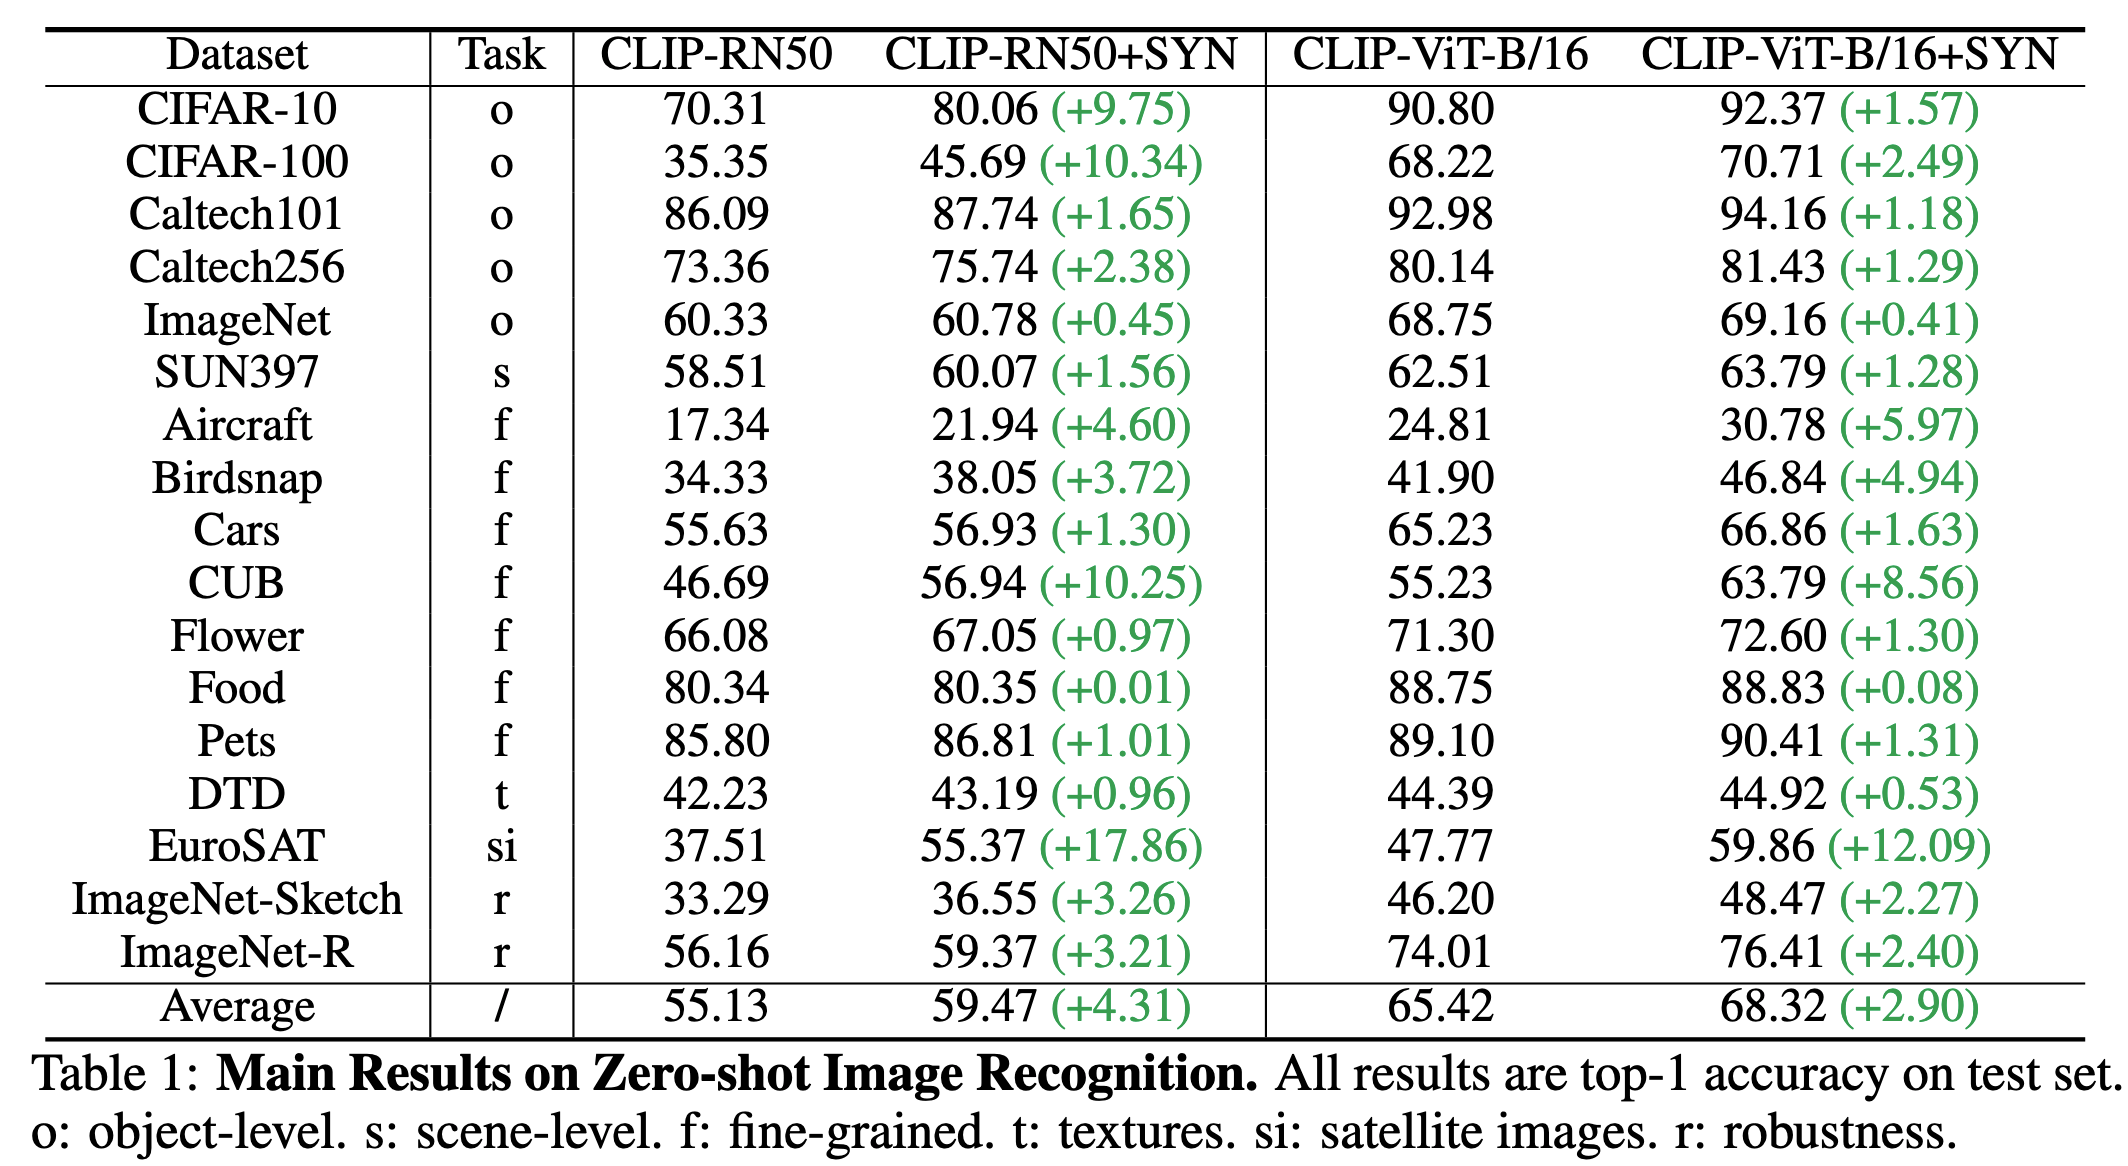
\includegraphics[width=0.70\linewidth]{figs/syn_aug_results.png}
      \caption{\scriptsize Improvement in classification performance when using synthetic data augmentation~\parencite{heSYNTHETICDATAGENERATIVE2022}.}
    \end{figure}
    \bottomleftrefs
  \end{frame}
  \end{refsection}

  \begin{refsection}
    \begin{frame}{Diffusion-based Synthetic Data Augmentation is Superior}
      \begin{figure}
        \centering
        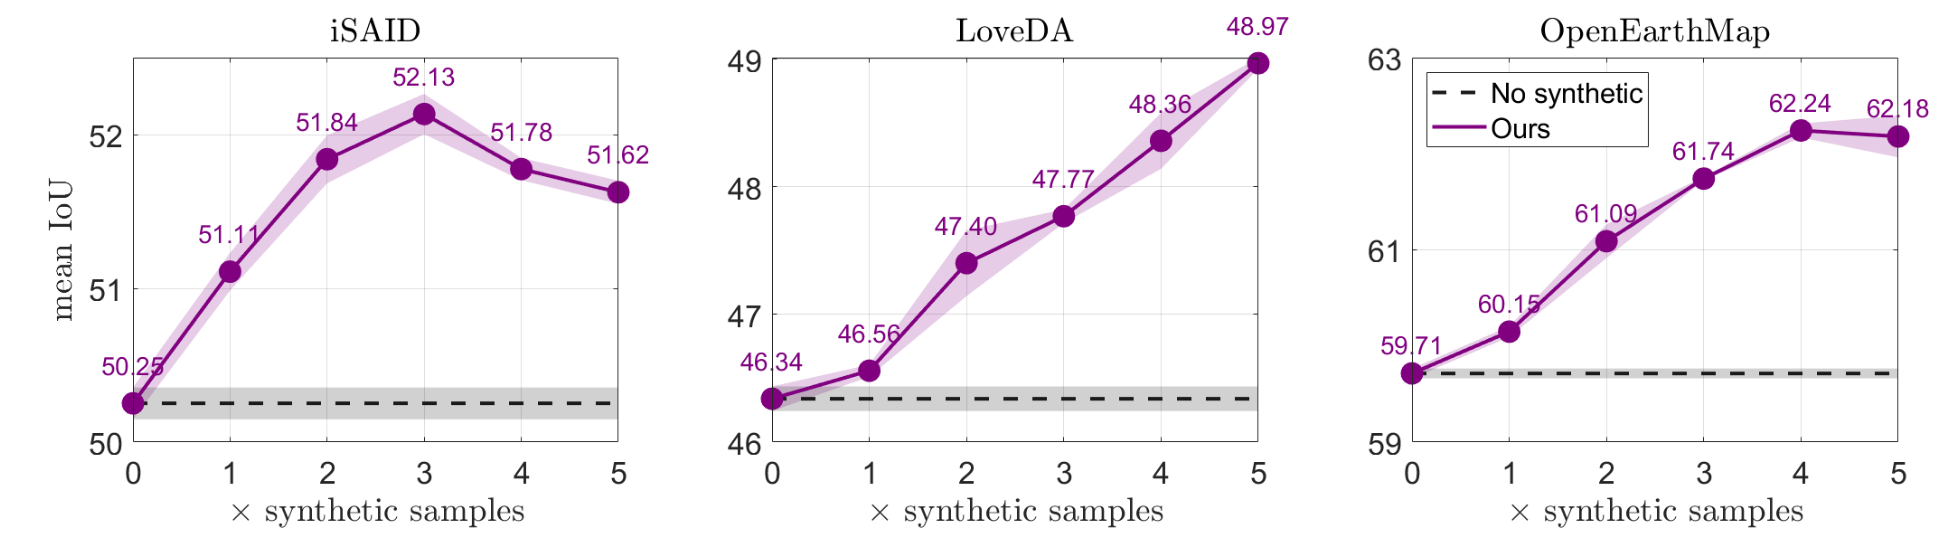
\includegraphics[width=0.7\linewidth]{figs/satsynth_comparison.png}
        \caption{\scriptsize Table from SatSynth: Diffusion-based synthetic data augmentation achieves higher segmentation accuracy compared to classical augmentation~\parencite{tokerSatSynthAugmentingImageMask2024}.}
      \end{figure}
      \vspace{-2.5em}
      \begin{table}[]
        \centering
        \caption[]{\scriptsize Quantitative comparison: mean IoU on iSAID~\parencite{waqas2019isaid} dataset.}
        \scriptsize
        \setlength{\tabcolsep}{2.5pt}
        \begin{tabular}{@{}l|cccc@{}}
        \toprule
        \textbf{No add.} & \textbf{Ours} & \textbf{Cutout~\parencite{devriesImprovedRegularizationConvolutional2017}} & \textbf{CutMix~\parencite{yunCutmixRegularizationStrategy2019}} & \textbf{Copy-Paste~\parencite{ghiasiSimpleCopyPasteStrong2021}} \\
        \midrule
        50.25 & \textbf{51.11} & 50.47 & 50.60 & 50.51 \\
        \bottomrule
        \end{tabular}
      \end{table}
    
      \bottomleftrefs
    \end{frame}
    \end{refsection}
    
% \begin{frame}[allowframebreaks]{References}
%   \printbibliography
% \end{frame}